\documentclass{article}
\usepackage[utf8]{inputenc}

\title{Hilos}
\author{Chrsitian Gallego Chaverra}
\date{July 2020}

\usepackage{natbib}
\usepackage{graphicx}

\begin{document}

\maketitle

\section{¿Que son los Hilos?}
Podemos definir un hilo de procesamiento como el flujo de control de datos de un programa. Es un medio que permite administrar las tareas de un procesador y de sus diferentes núcleos de una forma más eficiente. Gracias a los hilos, las unidades mínimas de asignación, que son las tareas o procesos de un programa, pueden dividirse en trozos para así optimizar los tiempos de espera de cada instrucción en la cola del proceso. Estos trozos se llaman subprocesos o threads.
Dicho de otra forma, cada hilo de procesamiento contiene un trozo de la tarea a realizar, algo más simple de realizar que si introducimos la tarea completa en el núcleo físico. De esta forma la CPU es capaz de procesar varias tareas al mismo tiempo y de forma simultánea, de hecho, podrá hacer tantas tareas como hilos tenga, y normalmente son una o dos por cada núcleo, como se muestra en la figura 1. En los procesadores que tienen por ejemplo 6 núcleos y 12 hilos serán capaces de dividir los procesos en 12 tareas distintas en lugar de solamente 6\cite{intro}.

\begin{figure}[h!]
\centering
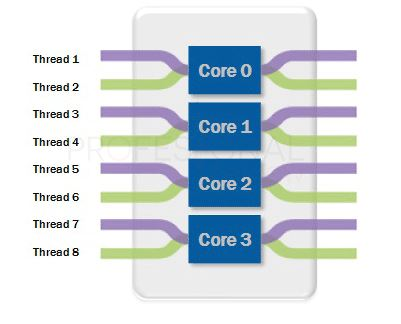
\includegraphics[scale=0.7]{hilos.JPG}
\caption{Hilos de un procesador.\cite{intro}}
\label{fig:hilos}
\end{figure}

\section{Tipos de hilos}
A nivel practico los hilos pueden ser implementados a nivel de usuario o a nivel de kernel.
A nivel de usuario son implementados en alguna librería. Estos hilos se gestionan sin soporte del SO, el cual solo reconoce un hilo de ejecución. Los hilos a nivel de usuario tienen como beneficio que su cambio de contexto es más sencillo que el cambio de contexto entre hilos de kernel. A demás, se pueden implementar aún si el SO no utiliza hilos a nivel de kernel.
Para los hilos a nivel de kernel es el SO quien planifica y gestiona los hilos. Se reconocen tantos hilos como se hayan creado. Los hilos a nivel de kernel tienen como gran beneficio poder aprovechar mejor las arquitecturas multiprocesadores, y que proporcionan un mejor tiempo de respuesta, ya que si un hilo se bloquea, los otros pueden seguir ejecutando.
Existen tres formas para relacionar los hilos a nivel de kernel y los de usuario.\cite{hker}

\subsection{Modelo Mx1(Many to one)}
El modelo asigna múltiples hilos de usuario a un hilo del kernel, como se muestra en la figura 2. Este caso se corresponde a los hilos implementados a nivel de usuario, ya que el sistema solo reconoce un hilo de control para el proceso.  Tiene como inconveniente que si un hilo se bloquea, todo el proceso se bloquea. También, dado que solo un hilo puede acceder al kernel cada vez, no podrán ejecutarse varios hilos en paralelo en múltiples CPUs.

\begin{figure}[h!]
\centering
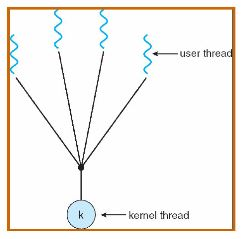
\includegraphics[scale=0.7]{hilos1.JPG}
\caption{Modelo Mx1.\cite{hker}}
\label{fig:hilos1}
\end{figure}

\subsection{Modelo 1x1 (one to one)}
El modelo asigna cada hilo de usuario a un hilo del kernel, como se muestra en la figura 3. Proporciona una mayor concurrencia que el modelo anterior, permitiendo que se ejecute otro hilo si uno se bloqueó.  Tiene como inconveniente que cada vez que se crea un hilo a nivel de usuario, se crea un hilo a nivel del kernel, y la cantidad de hilos a nivel del kernel están restringidos en la mayoría de los sistemas. 

\begin{figure}[h!]
\centering
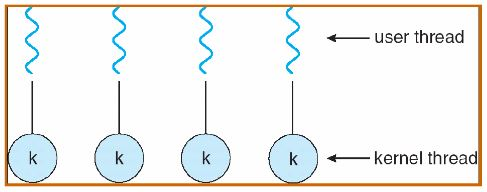
\includegraphics[scale=0.7]{hilos2.JPG}
\caption{Modelo 1x1.\cite{hker}}
\label{fig:hilos2}
\end{figure}

\subsection{Modelo MxN (Many to Many)}
El modelo multiplexa muchos hilos de usuario sobre un número menor o igual de hilos del kernel, como se muestra en la figura 4. Cada proceso tiene asignado un conjunto de hilos de kernel, independientemente de la cantidad de hilos de usuario que haya creado. El usuario puede crear tantos hilos como necesite y los hilos de kernel pueden ejecutar en paralelo. Asimismo, cuando un hilo se bloquea, el kernel puede planificar otro hilo para su ejecución.  Entonces, el planificador  a nivel de usuario asigna los hilos de usuario a los hilos de kernel, y el planificador a nivel de kernel asigna los hilos de kernel a los procesadores

\begin{figure}[h!]
\centering
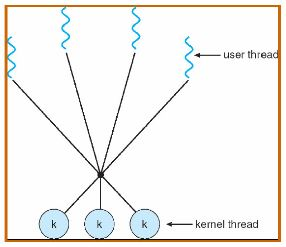
\includegraphics[scale=0.7]{hilos3.JPG}
\caption{Modelo MxN.\cite{hker}}
\label{fig:hilos3}
\end{figure}

\subsection{Multihilo o Multithreading}
En la arquitectura de computadores , multihilo es la capacidad de una unidad central de procesamiento (CPU) (o un único núcleo en un procesador multi-núcleo ) para ejecutar varios procesos o hilos simultáneamente, apoyada por el sistema operativo. Cuando los sistemas de multiprocesamiento incluyen múltiples unidades de procesamiento completas en uno o más núcleos, multihilo pretende aumentar la utilización de un solo núcleo mediante el uso de paralelismo a nivel de hilo\cite{para1}, así como el paralelismo a nivel de instrucción\cite{para2}. Como las dos técnicas son complementarias, a veces se combinan en sistemas con una CPU multithreading múltiple y con CPUs con múltiples núcleos multithreading\cite{multi}.

El ejemplo de la implementación en c++ se encuentra adjunto en el repositorio.

\bibliographystyle{plain}
\bibliography{references}
\end{document}
